\subsection{Resultados De Escenario Experimental A}

El objetivo de las pruebas realizadas en el presente escenario experimental, era validar que, los procesos implementados, efectivamente realizaran la adaptación de las aplicaciones desde un estado de completa falla, en donde ninguno de los datos necesarios estuviera presente.

Siguiendo los pasos definidos en la sección \ref{sec:EscenarioExperimentalA}, se realizó el despliegue de los servicios base de Smart Campus UIS, al igual que \textit{Bran} y \textit{DoThing}. Como se presenta en la figura \ref{fig:LookerStart}, se registró el estado de referencia al agregador tras validarlo usando \textit{Lexical}, y se fijaron las directivas a usar para la adaptación de la arquitectura.

\begin{figure}[H]
    \centering
    \caption{Aplicación y directivas registradas en Bran}
    \label{fig:BranStart}
    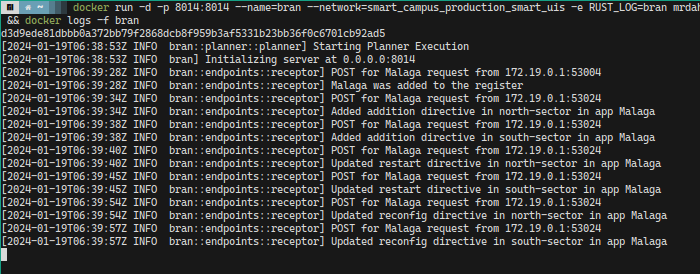
\includegraphics[width=\linewidth]{images/BranStart.png}
    \vspace{-4mm}
\end{figure}

Una vez se inició el servicio \textit{Looker}, como se ve en la figura \ref{fig:LookerStart}, este empezó a evaluar el estado de la aplicación; que al no tener ningún tipo de reporte de algún componente, entró directamente en estado de falla. 

\begin{figure}[H]
    \centering
    \caption{Looker evalúa el estado de la aplicación}
    \label{fig:LookerStart}
    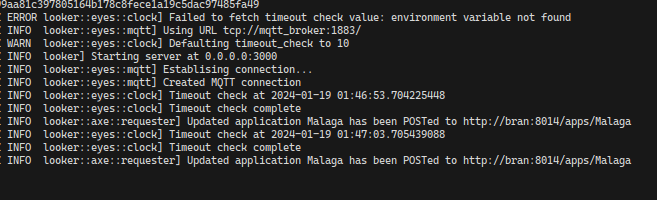
\includegraphics[width=\linewidth]{images/LookerStart.png}
    \vspace{-4mm}
\end{figure}

El estado observado, se reportó a \textit{Bran}, el cual, realizó el recorrido para identificar los puntos de falla de la aplicación. Como se observa en la figura \ref{fig:BranPlan}, como era de esperar, los tres requerimientos definidos en cada una de las locaciones estaba en estado de falla. Al no haber componentes reportando datos, como era de esperarse, se definieron acciones \textit{Addition} para todos los componentes de la aplicación. 

\begin{figure}[H]
    \centering
    \caption{Bran identifica los problemas y establece las acciones}
    \label{fig:BranPlan}
    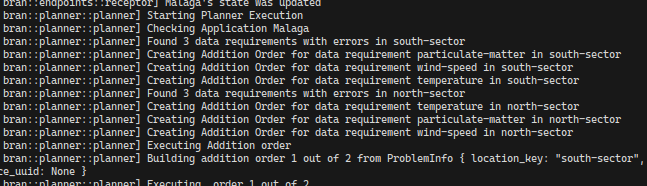
\includegraphics[width=\linewidth]{images/BranPlanning.png}
    \vspace{-4mm}
\end{figure}

A partir de las acciones, se crearon las órdenes para ejecución usando las directivas como base. Cada una de estas se envió a \textit{DoThing}, el cual realizó 

\begin{figure}[H]
    \centering
    \caption{DoThing ejecuta las acciones establecidas por Bran }
    \label{fig:DoThingDoing}
    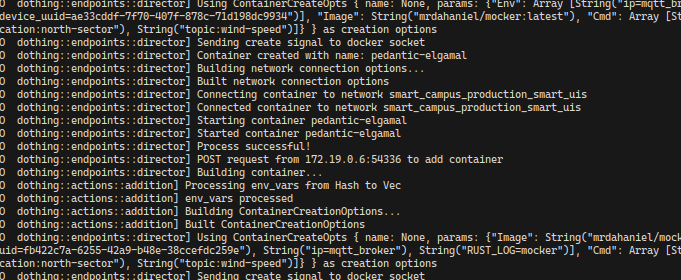
\includegraphics[width=\linewidth]{images/DoThingDoing.png}
    \vspace{-4mm}
\end{figure}

\begin{figure}[H]
    \centering
    \caption{Bran identifica otros problemas en la aplicación}
    \label{fig:BranPlan2}
    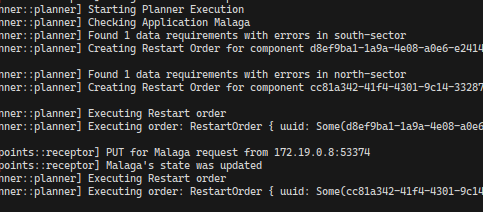
\includegraphics[width=\linewidth]{images/BranRestarting.png}
    \vspace{-4mm}
\end{figure}

\begin{figure}[H]
    \centering
    \caption{Bran establece acciones de reconfiguración para adaptar la aplicaciónj}
    \label{fig:BranPlan3}
    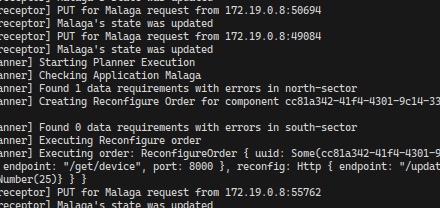
\includegraphics[width=\linewidth]{images/BranReconfiguring.png}
    \vspace{-4mm}
\end{figure}



